% !TEX root = ./paper.tex

In this section, we evaluate \tcpls with several experiments. First, we evaluate the raw performance of our \tcpls prototype (Sec.~\ref{sec:perf}). Then, we report how \tcpls interacts with middleboxes in a controlled environment in  Sec.~\ref{sec:middlebox}. We then emulate, using Mininet~\cite{handigol2012reproducible}, more complex scenarios involving
Failover (Sec.~\ref{sec:eval_failover}), Application Connection Migration
(Sec.~\ref{sec:app-migration}) and Bandwidth Aggregation  (Sec.~\ref{sec:bwaggr}).

For the two first experiments of our \tcpls prototype (Sec.~\ref{sec:perf} and~\ref{sec:middlebox}), we use the testbed depicted in Fig.~\ref{fig:perf_testbed}. It consists of three servers equipped with Intel Xeon CPU E5-2630 2.40GHz, 16~GB RAM, running Debian with Linux 5.9 and 5.7 kernels. Two of these machines are used as, respectively, Client and Server, while the third one is used as a router or a middlebox, depending on the scenario. Each machine is equipped with an Intel XL710 2x40~Gbps NIC. For all measurements, with all implementations, we use a  single thread on each machine to run the client and server.

\begin{figure}[!t]
	\begin{center}
		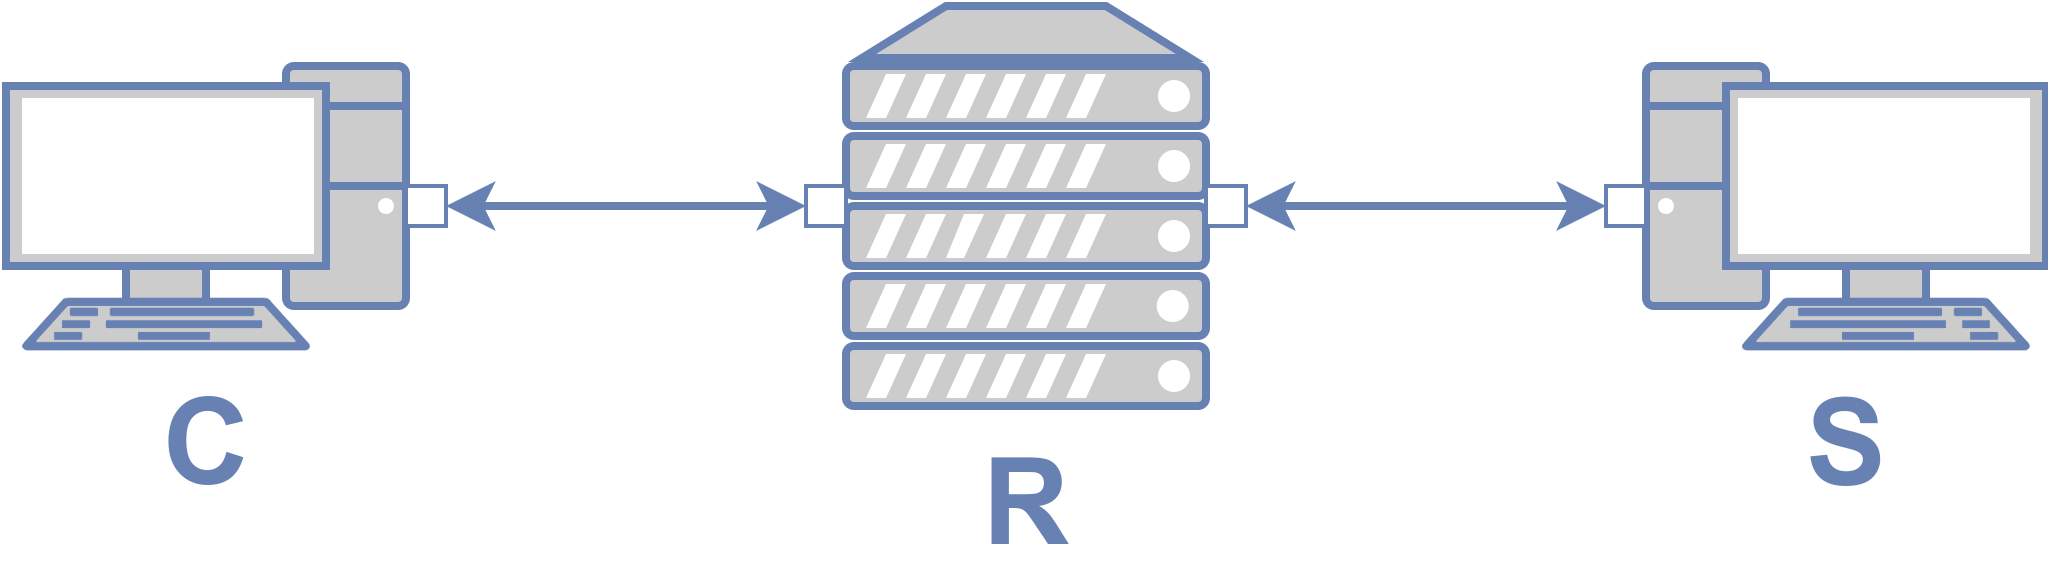
\includegraphics[width=.6\columnwidth]{figures/testbed.png}
	\end{center}
	\caption{Performance Measurements Setup. C = Client. S = Server. R =
	Router/Middlebox.}
	\label{fig:perf_testbed}
\end{figure}

In the emulated experiments of Sec.~\ref{sec:eval_failover},
\ref{sec:app-migration} and \ref{sec:bwaggr}, we use a Mininet  network~\cite{handigol2012reproducible} composed of a client and a server, both
dual-stacks. The IPv4 and IPv6 paths are completely disjoint in this emulated
network, each offering 25~Mbps and 10~ms latency if not stated otherwise.



%Our objective is to evaluate whether our design and implementation are indeed
%fast, flexible and does not conflict with several commercial and open-source
%middleboxes. Moreover, we expect to showcase and compare TCPLS's functionalities
%such as the App-level connection migration, the failover mechanism or the
%bandwidth aggregation capability. We discuss them against the state
%of the art designs, such as mvfst~\cite{mvfast}, quicly~\cite{quicly},
%msquic~\cite{msquic}, MPTCP~\ref{mptcp}, pquic~\cite{pquic},
%quic-go~\cite{quic-go} and MPQUIC~\ref{mpquic}.

%TODO do we also evelatuate security? with a simple proof and discussion?

%To evaluate \tcpls's functionalities, we rely on reproducible network
%experimentations with Mininet~\cite{mininet}. Our objective is to compare the
%behaviour of \tcpls with the state of the art, and to make it easily
%reproducible for future works, as the quic implementations continue to evolve.


\subsection{Raw Performance} \label{sec:perf}
In our first experiment, we demonstrate that \tcpls can be implemented at a low
cost compared to \tcp and \tls while offering better raw performance than
several \quic implementations. To this end, we use the physical testbed
presented in Fig.~\ref{fig:perf_testbed} and run throughput measurements for
large transfers with \tcp/\tls, \tcpls and three \quic implementations.
The results are reported in Fig.~\ref{fig:perf} with the bandwidth
in gigabits per second and packets per second obtained for each test.
Each bar corresponds to the median measurement over 10 seconds of stable
throughput. A preliminary test in our testbed shows that a single \tcp connection can saturate the 40~Gbps link when setting the MTU to 9000 bytes. With a 1500-byte MTU, a single \tcp connection reaches 22~Gbps. We also benchmarked the AES128-GCM-SHA256 cipher with in-memory 16,384-byte \tls records and observed that decryption in our client reaches 24.59~Gbps while encryption on our server reaches 13.62~Gbps.

%With this first experiment, we demonstrate that \tcpls can be implemented at a
%low cost compared to \tcp and \tls while
%The first question we want to answer is whether \tcpls can compete with the
%traditional \tls over \tcp stack. We also compare our \tcpls prototype with
%different \quic implementations.

\textbf{\tcp/\tls}. To get a fair reference point, we first evaluate \tls over
\tcp using \texttt{picotls} with the AES128-GCM-SHA256 cipher at the commit
starting our fork. We also manually configured the receiving and sending buffer size to match the ones we use internally in \tcpls. This modification fixes fragmentation and unnecessary copies of received \tls records that could occur and improves by $\approx 40\%$ the throughput of \texttt{picotls}'s measurement client. Our \tcpls prototype avoids these mistakes by design by offering to the application developers a transport API preventing them. % adversely affecting the %throughput.
With the fix, we can observe that \tcp/\tls reaches 10.3~Gbps with a 1500-byte MTU and 12.6~Gbps with a 9000-byte MTU. Both leverage \tcp Segmentation Offload (TSO), which is a feature commonly enabled on high-speed NICs.

\textbf{\tcpls}.
To benchmark \tcpls, we use a simple application performing large
memory-to-memory transfers over a \tcpls session using a single stream, also
%For all the \tcpls measurements, we use a custom application that performs
%large memory-to-memory transfers over a \tcpls session using a single stream.
%\tcpls is
configured to use the AES128-GCM-SHA256 cipher.
%Fig.~\ref{fig:perf}
%provides the throughput as measured in our testbed. We report both the
%bandwidth in
%gigabits per second and packets per second. Each bar in Fig.~\ref{fig:perf}
%corresponds to the median measured over 10 seconds of stable throughput. The
%bottom bar (labeled ``\tcpls tso on mtu 9000'') is the highest median
%throughput
%that we measured with \tcpls: 12.4~Gbps. This result was obtained with jumbo
%frames (i.e., 9000 bytes MTU) and using \tcp Segmentation Offload (TSO) on the
%NICs. TSO is a standard feature that is enabled by all high-speed NICs.  Note
%that on
%both machines, encryption is $\approx 40\%$ slower than decryption.
%which explains the gap between TCPLS and raw TCP.
%The next bar (labeled ``\tcpls tso on'') shows that with TSO and standard frame
%size (1,500 bytes MTU), the throughput still reaches 10.84 Gbps. These
%results should be compared with the 22~Gbps \tcp reaches in the same
%environment using \texttt{iperf} but without any encryption.
We first compare \tcpls without the transport services presented in Sec.~\ref{sec:transport-services}. We can observe that \tcpls reaches similar throughput than \tls/\tcp over both MTU. The small advantage of \tcpls at an MTU of 1500 bytes may be attributed by implementation differences in the two benchmarks tools. \tcpls has thus a similar throughput than \tcp/\tls when using the base protocol. %We now evaluate the cost of the transport services.


%the shows several interesting results. First, while offering similar (and more)
%capabilities than what QUIC is providing today,
%\tcpls is also more than twice faster than the strongest evaluated QUIC
%implementation (quicly) over CPU limited experimentations. We evaluate \tcpls

We then evaluate the cost of enabling Failover, which adds \tcpls-record-level
acknowledgments. % of adding the \tcpls-level
%acknowledgments
%described in Section~\ref{failover} to support failover.
% Thanks to these acknowledgments, \tcpls can support failover.
Our measurements show that Failover has a small impact on raw throughput as
\tcpls reaches 9.66~Gbps with a $1500$ bytes MTU. This is due to an increase in control records that are exchanged during the file transfer and additional buffer management within \tcpls. This impact could be reduced by lowering the number of record acknowledgments, which could further improve the throughput with an MTU of 9000 bytes. We leave finding the optimal acknowledgment frequency as future work.
%From a performance viewpoint, they increase the
%number of control records
%exchanged and the number of system calls.
%Our prototype currently sends a
%\tcpls-ack for every
%16 received records.
%\todo{Commenter Failover mtu 9000}


%% We also compared \tcpls's native bandwidth aggregation using two streams with a
%% single stream produced by our \tcpls client on the top of the \mptcp kernel
%% creating two \mptcp subflows. Our \tcpls scheduler is a simple round-robin. The
%% \mptcp scheduler is the lowest-RTT scheduler enabled by default. Both
%% measurements are taken over the same 0.94.7 \mptcp kernel with a path MTU of
%% 1,500, in which \mptcp is disabled when the \tcpls native experiment is
%% performed.  Surprisingly, \tcpls's native bandwidth aggregation outperforms
%% \mptcp. Both experiments are CPU limited, and suffers from a raw throughput
%% degradation compared to the single-path experiment. \tcpls's reordering is
%% implemented with an heap~\cite{heap-github} highly efficient in
%% resizing, but the main factor holds on the number of packets treated for
%% reordering. Inside \mptcp, it reorders packets of $1,460$ bytes, even when those
%% packets are part of the \textit{same} record. This information is only available
%% at the \tcpls level, which reorders large chunk of data instead (max payload is
%% $16,384$ bytes). This is somehow similar to the $Jumbo$ frames optimization goal:
%% pushing larger data packets to reduce the number of times the same code is
%% called.  Besides
%% \tcpls's native  multipath uses the \tcp optimized stack, which together offer a
%% strong secure bandwidth aggregation solution.

Finally, we evaluate the cost of using coupled streams over several \tcp connections.
%Our next step was to evaluate the cost of the multi-connections stream
%steering feature of \tcpls.
We configured \tcpls to use IPv4 and IPv6 as separate network paths and start a
\tcp connection on each path.
%We configured IPv4 and IPv6 addresses on the Client and the Server and created
%a \tcpls session that uses two \tcp connections.
The \tcpls server sends the records over the two \tcp connections in a
round-robin manner. The \tcpls client receives and reorders the records using
an efficient heap.
%Our Server steers the data in
%the \tcpls streams using a
%round-robin scheduler to send the records over the available connections.
%This is not the best scheduler for sending data over multiple
%paths~\cite{paasch2014experimental} since it will force the
%receiver to reorder the received records.
Our measurements show that coupling when two streams in our testbed, \tcpls reaches a throughput of 8.8~Gbps, i.e. less than 10\% below Failover.

\begin{figure}[!t]
  \begin{center}
    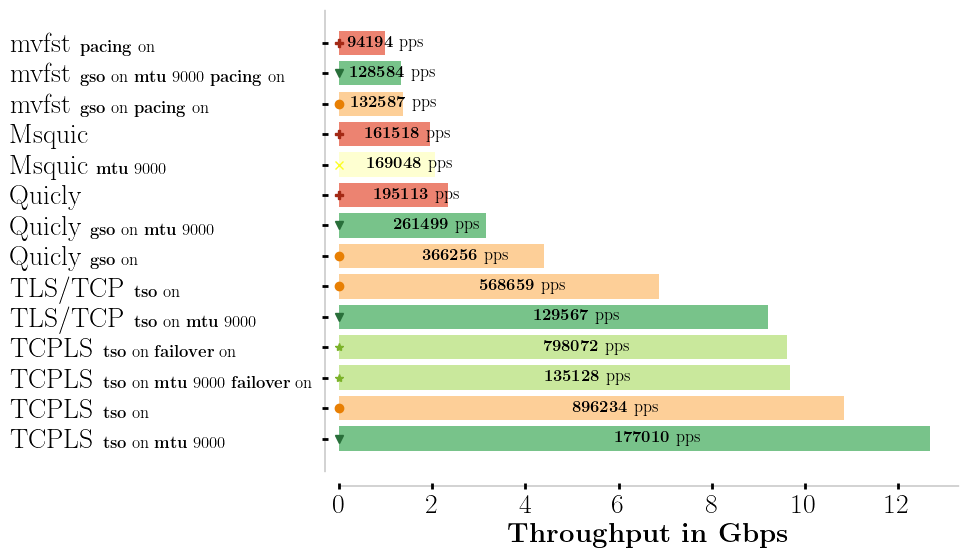
\includegraphics[width=\columnwidth]{figures/perf_analysis.png}
  \end{center}
  \caption{Throughput comparison between \tcpls, \tcp/\tls, and three \quic
  implementations.
    %Single-thread client/server for all implementations.
    The \tcpls prototype is faster than several major \quic implementations while offering a superset of transport services and similar flexibility.}
  \label{fig:perf}
\end{figure}


%in four different settings: with a path mtu of 1500 or 9000, and with failover
%enabled or not. The failover functionality is an internal stack feature that
%provides session reliability, which increases the number of syscalls that TCPLS
%makes by exchanging TCPLS-level record acknowledgments. We currently send an
%ac%k for throughput at the price of a slower recovery in case of network
%failure.

%\paragraph*{\tcpls vs. \tls/\tcp} We now compare the performance of \tcpls with
%the traditional \tls over \tcp stack. To have a fair comparison, we use
%\texttt{picotls}'s perf client/server implementation with the same commit as
%our
%initial fork for \tcpls. Fig.~\ref{fig:perf} shows that \tls/\tcp provides a
%lower performance than \tcpls with regular and jumbo frames. This can be
%explained by the receiving buffer size provided to \texttt{read()}, which is
%hardcoded to 16,384 bytes in \texttt{picotls}'s perf client. This
%implementation
%choice results in fragmentation on the receiver and prevents it from using
%efficiently the
%zero-copy code path provided by the library. Our \tcpls implementation uses a
%larger read buffer with auto-tuning
%and benefits from zero-copy. At first, one may consider this as an unfair
%comparison. \tcpls's design is an attempt to solve a common mistake. Indeed,
%in our \tcpls implementation,
%the application developers cannot touch \texttt{read()}'s interface. This
%implies that an application developer cannot misuse the relationship between
%\tls and \tcp by creating fragmented records and doing unnecessary copies to
%handle those fragments. \tcpls's design and implementation try to prevent
%fragmentation by, first, having a sufficiently large read buffer size. Second,
%\tcpls deciphers a record when it has received the entire content.
%\tls libraries provide \tls/\tcp record fragmentation as a usability
%feature that spares the application developers from taking into account all
%\tls
%details, at the cost of lower performance. With \tcpls, application developers
%can ignore \tls details without misusing the interface, which is why
%this comparison is interesting. \tcpls constrains the application developer to
%use the buffer type provided by the API, but offers zero-copy deciphered
%records
%in return. Note, however, that the main culprit for the lower \tls/\tcp result
%is the read buffer size. Increasing the read buffer size of the perf client
%using \texttt{picotls} fills the performance gap with \tcpls.

%\todo{OB: pas sur que la suite est nécessaire} Moreover, but this has not
%yet been implemented, it could be interesting to match the TLS record size to
%the congestion window to deliver faster the data to the application when the
%network is congested.

\textbf{\quic}.
%Although \quic~\cite{draft-ietf-quic-transport} is a young protocol, there are
%already more than a dozen
%implementations~\cite{marx2020same,quicimplem,yang2020making} under active
%development.
We evaluate three representative \quic implementations in our testbed:
Facebook's \mvfst~\cite{mvfst-github,Joras_mvfst}, Microsoft's
\msquic~\cite{msquic-github}, and Fastly's \quicly~\cite{quicly-github}. They
are intended for production use and include throughput measurement applications.
Furthermore, \mvfst and \quicly support Generic Segmentation Offload (GSO),
which offloads \udp segmentation and checksum computation to the kernel and NICs.
%We use the
%implementation's benchmarking application as
%is, exploiting the optional arguments provided by their interface to increase
%the throughput but drawing the line there.
%We do not modify the \quic
%implementations and use their default cipher.
We configured the \quic implementations to the most comparable setting as
\tls/\tcp and \tcpls. That is, we changed the cipher and set the CUBIC
congestion controller when available.
% to the same ones used by
%\tcpls when they did
%not adversely
%affect \quic's performance too much. For example, several congestion
%controller
%are implemented in the \quic stacks but changing the default
%one often led to lower performance or unstable throughput.

The results obtained show that \tcpls compares favorably with the tested \quic implementations. The fastest \quic implementation is \quicly, with GSO and a 1500-byte MTU, it reaches 4.4~Gbps. \tcpls with TSO is twice faster with the same CPU usage and similar receiving buffer sizes. Surprisingly, \quicly's performance decreases with jumbo frames but is still faster than without GSO.  \msquic reaches 1.96~Gbps while \mvfst was slower despite GSO.
%The results are quite good for \msquic and \quicly.
%Indeed, since \msquic does not yet use GSO, the speed of
%this implementation is fundamentally limited by the speed of the Linux Kernel's
%interface with UDP.
The lower performance of \quic implementations can be explained by several
factors originating from the Linux \udp interface and \quic design.
%\quic is known to have several performance shortcomings compared
%to \tls/\tcp, in short: 1) \quic relies on $sendmsg$/$recvmsg$ which allows 1
($i$) Early \quic implementations use \texttt{sendmsg}/\texttt{recvmsg},
exchanging one packet at a time with the kernel.
($ii$) GSO is often not supported by the NIC and implemented in the kernel,
unlike TSO.
($iii$) Pacing is implemented in userspace.
($iv$) Acknowledgments are handled in userspace, increasing further the number
of context switches.
($v$) \quic packets are smaller units than \tls records for encryption and
decryption.
%packet at a time, 2) 1350-byte
%plaintext encryptions (\quic) vs 16384-byte plaintext encryption for \tls and
%\tcpls (higher is better),
%3) Pacing in userspace for \quic, 4) Segmentation in the kernel for \quic
%using GSO not as good as TSO
%(hardware, on the NIC for \tls/\tcp and \tcpls), 5) transport
%acknowledgments in userspace for \quic increasing the number of
%context-switches. While some of these shortcomings may
%still be improved, several are carved in \quic's choice to use UDP.
While there are ongoing works to improve $i$, $ii$, and $iii$~\cite{udp-gso-pacing}, it is likely that performance parity will require more offload capabilities, which could lessen the flexibility of \quic. From a security standpoint, assuming NICs are opaque components of the network and not part of the user stack, it would be less compliant to the end users threat model.
%It would also uncompliant regarding the end users'
%threat model
%(untrusted network, and we assume the NICs are a component of the network and
%not part of the user's stack).
%There isn't likely enough room to match \tcpls performance
%without offloading everything, which inherently breaks \quic's flexibility
%argument


%QUIC is young protocol, and all implementations are in active development, with
%different states for their available features and optimizations. For example,
%none of the implementations were able to take advantage of a path mtu larger
%than 1500, and it even degraded the performance in the case of quicly. Two of them
%(quicly and mvfst) have implemented the support for \texttt{gso} leading in the
%case of quicly to more than 4 gb/s of throughput with a udp payload length
%configured to match TCP (1460).


%We perform a throughput evaluation of \tcpls and compare it to several major
%QUIC implementations: mvfst~\cite{} from Facebook, msquic~\cite{} from Microsoft
%and quicly~\cite{} from Fastly. Our choice of QUIC implementations was mainly
%influenced by the availability of a client/server perf tool specifically
%engineered for a throughput evaluation. A second criterion was the advancement
%of the implementation and the quality of the code. We hope to avoid most of the
%bugs negatively impacting their results by selecting the QUIC implementation
%that show advanced features and testings. A third criterion was the development
%language used. \tcpls is written in C, and we prefer to compare it against QUIC
%implementation written in a language compiled by clang or gcc. Mvfst, msquic
%and quicly meet these criteria.


\subsection{Middlebox Interference}
\label{sec:middlebox}

We have tested \tcpls against different opensource and commercial stateful
firewalls and proxy implementations (i.e., pfSense, IPFire, Cisco ASAv,
mitmproxy) and found no unexpected interference. Stateful filtering and stateful
packet inspection policies did not impact the \tcpls handshake and transparent
\tls proxy successfully triggered \tcpls fallback to \tls/\tcp. Still, the security appliances that block \tls 1.3 or some of its features~\cite{lee2019matls,Bock_China,raman2020measuring} would also block \tcpls.
%pervasive monitoring allows for configurable TLS extensions blocking
%\cite{rfc7258}. This is handled properly by \tcpls fallback mechanism.

When faced with middleboxes that modify \tls 1.3~\cite{Bock_China,raman2020measuring}, only one type of \tcpls messages can be impacted. The client \tls extensions, that are integrity-protected but not confidential, can be modified by these middleboxes. They contain messages such as \hello, \join, \textit{SESSID}, and \textit{COOKIE} presented
in Sec.~\ref{sec:transport-services}. Other messages conveyed in encrypted \tls records cannot be distinguished or tampered with. When a client opens a \tcpls session through a \tls terminating proxy not supporting \tcpls, it replies
with a \textsc{ServerHello} message omitting the \hello extension. Then, the client can implicitly fall back to \tls and continue with the handshake.

Some legacy \tls server implementations do not implement the \tls specification properly and might abort connections when receiving unknown \tls extensions. Similar behavior has been observed in overly restrictive stateful firewalls. To ensure connectivity in the presence of such policies, \tcpls implements an explicit fallback mechanism. If a client receives a \tcp \rst in response to the \tcpls \textsc{ClientHello} or no response, it tries negotiating a regular \tls connection after a timeout fired. In the same manner, a \join extension might be blocked on a path when joining connections. In this case, the subflow
attachment is canceled, and the application is notified to react appropriately, e.g., to cancel the migration.

A more complete evaluation of middlebox interference would require measurements
in various operational networks that include such
devices~\cite{honda2011still,raman2020measuring,o2016tls}. This is
outside the scope of this paper and left for further work.

%We tested \tcpls against opensource and commercial stateful firewalls and proxy
%implementations and (i.e., pfSense, IPFire, Cisco ASAv, mitmproxy) and found no
%interferences. Still, certain middlebox security appliances that implement
%pervasive monitoring allows for configurable TLS extensions blocking
%\cite{rfc7258}. This is handled properly by \tcpls fallback mechanism.


\subsection{Failover}
\label{sec:eval_failover}

Failover is designed to provide resilience to \tcpls connection failures. Network outages may happen for several reasons, e.g., middlebox interference or mobile clients losing one access network (LTE or Wi-Fi). We first discuss and compare the recovery time for different types of outages during a file transfer for \tcpls and \mptcp \footnote{Existing MPQUIC implementations~\cite{de2017multipath,de2019pluginizing} are not evaluated as detecting and reacting to network failures were not part of their prototypes.}.
We configure the client and the server with two interfaces, with one set to the
backup mode in the case of \mptcp, i.e., no subflows are opened on the backup
interface unless an issue is detected on the first interface. We consider two
types of outages: a middlebox blackholing all the traffic and the reception of a
spurious \rst. Fig.~\ref{fig:recovery} compares the goodput achieved by \mptcp and \tcpls over time when encountering these events.

\begin{figure}[!t]
  \begin{center}
    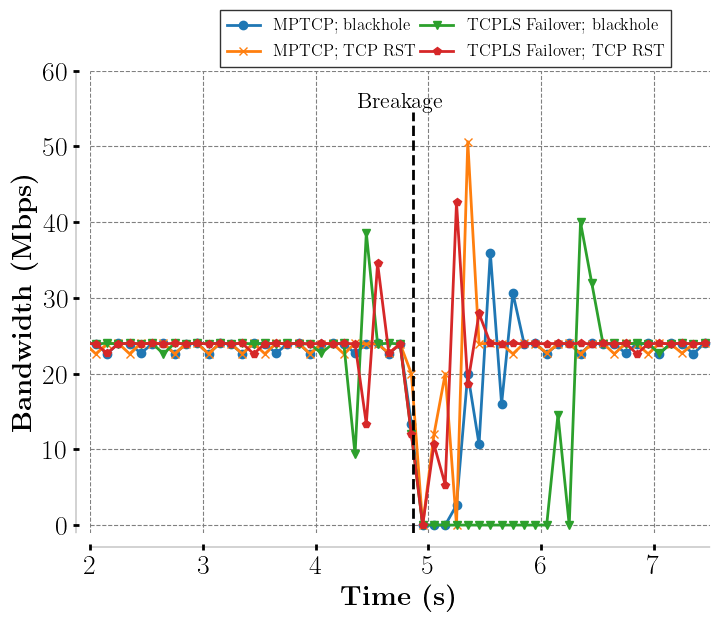
\includegraphics[width=.8\columnwidth]{figures/breakage_analysis.png}
  \end{center}
  \caption{Recovery delays of \tcpls compared to \mptcp during a single outage.}
  \label{fig:recovery}
\end{figure}

We can observe that upon reception of a \tcp \rst, both \tcpls and \mptcp react fast. This is an explicit signal they both act on quickly and resume the transfer. However, a network outage is more difficult to detect. Both stacks rely on timers to decide to switch paths. In the case of \tcpls, we configure a timer using the \tcp \texttt{User} \texttt{Timeout} option, which is set to $250~ms$ in our experiment. This value can also be chosen by the application according to specific use cases.
%(mp): (should) already been explained in sec. prototype
%When the server enables failover, it sets a timeout to protect
%the transfer. This option is sent in encrypted \tcpls records to
%indicate to the client \tcpls's stack that it should not wait more than $X ms$
%between successful reads of data, with $X$ a parameter of this option. For
%this experiment, the $USER\_TIMEOUT$ is set to $250~ms$.
When the timer expires, the client creates a connection over the other path and
joins it to the session. The server then replays the unacknowledged records.
Once these steps have succeeded, the transfer can continue. We can observe that
this process takes $\approx 1$ second to recover from this single outage in our
experiment.

\begin{figure}[!t]
  \begin{center}
    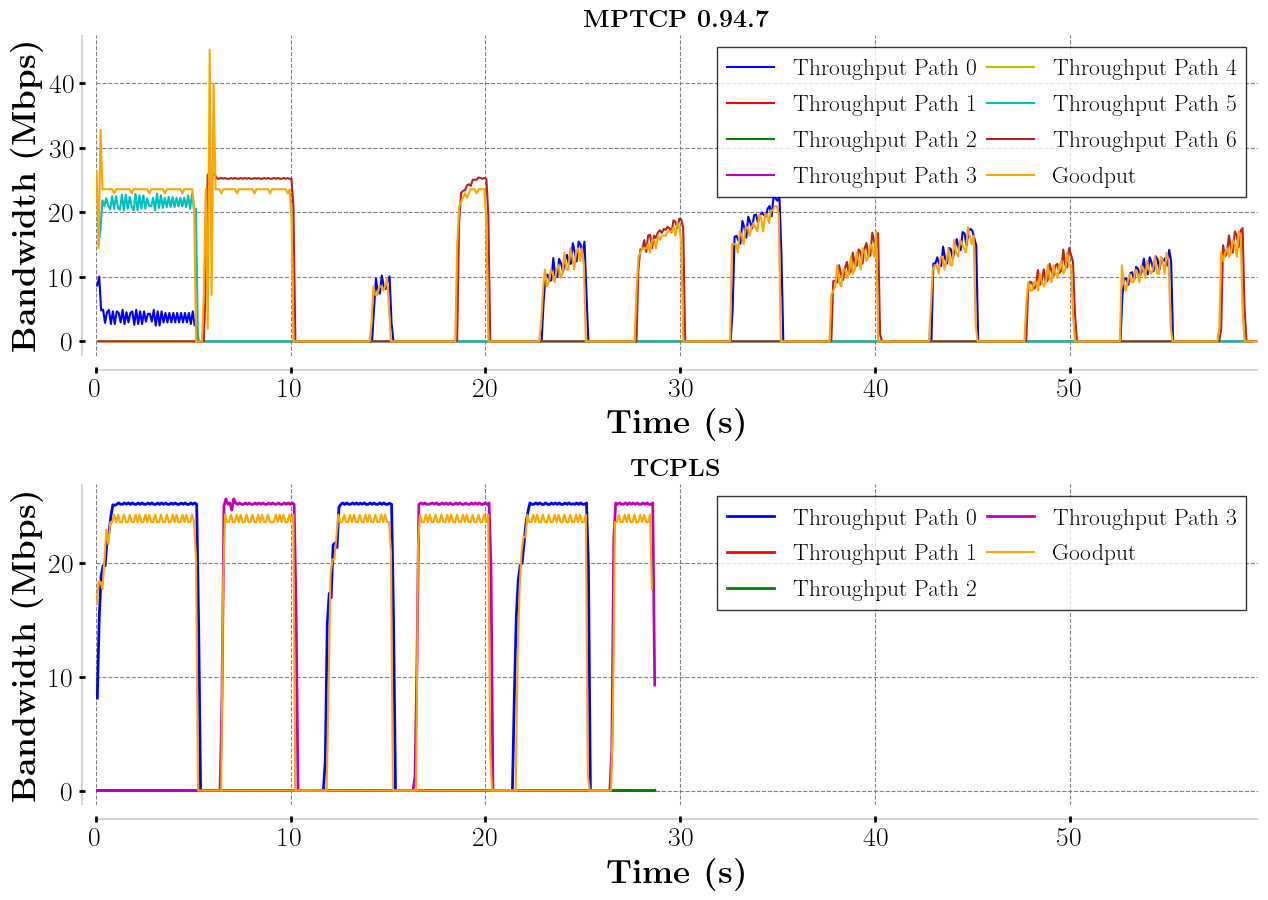
\includegraphics[width=\columnwidth]{figures/tcpls_mptcp.png}
  \end{center}
  \caption{\mptcp has difficulties to react to successive network outages during a 60MiB file download.
  \tcpls reacts quickly to such outages and complete the download faster.}
  \label{fig:failover}
\end{figure}

We now extend our first experiment by adding periodic outages during the
transfer in a 4-path network topology.
%The second experiment involves observing how different multipath
%implementations behave when several failures occur during a data transfer.
%We compared \tcpls with several multipath transport implementations: \mptcp,
%PQUIC with the
%multipath
%plugin~\cite{de2019pluginizing}, and MPQUIC~\cite{de2017multipath}.
%We do not report the results with PQUIC and MPQUIC as
%detecting and recovering from network failures were not part of these
%prototypes.
%We dug into these implementations and observed that they were not programmed
%to
%detect network failures and correctly switch the network path, thus we
%preferred to ignore those results.
\mptcp is a more mature multipath transport implementation that is maintained
and used in production. Fig.~\ref{fig:failover} compares how \mptcp and \tcpls recovers when three paths out of four are blackholed every five seconds. We rotate the working path so that each implementation has first to find it before recovering the transfer. We observe that \mptcp's default path manager performs well on the first failure. For the next ones, it requires several seconds to recover the right path.
%Besides, \mptcp seems to remember that something wrong
%happened, and enters a kind of congestion avoidance state until the end of the
%transfer. We may question this design choice, since many \tcp connections on
%the
%Internet have a shorter lifespan than 10 seconds (i.e., the time after which
%\mptcp should re-use a previously used path in this experiment).
We also tried injecting \tcp \rst instead of blackholing paths and \mptcp
indefinitely stalled after the second \rst. However, \tcpls finds the right path quicker and recovers the session in a short time similarly to the drop and \rst outage studied in Fig.~\ref{fig:recovery}. Moreover, since those connections are fresh, they can quickly use the available bandwidth.

\subsection{Application-level Connection Migration}
\label{sec:app-migration}

When there are multiple network paths, connection migration can be used by
applications to adapt to the changing network conditions based on application
metrics.

Applications can migrate their traffic from one network path to another using a few \tcpls API calls. Fig.~\ref{fig:conn_migration} shows the goodput obtained when performing such a migration during a file transfer with \tcpls. We do not compare \tcpls to \mptcp and \quic as none of their implementation offer this feature directly to applications. % using the
%API
%(i.e., the application decides
% when to migrate, and we expose a simplistic code flow to
%perform it).
In this experiment, we reuse the Mininet topology %introduced in
%Section~\ref{sec:bwaggr}%. We
and set a bandwidth of 30~Mbps on each path, a 40~ms round-trip-time for the IPv4 link, and 80~ms for the IPv6 link. Our test application downloads a 60~MB file and migrates once from the IPv4 to the IPv6 path and once again back to the IPv4 path.

%\todo{Est-ce necessaire? A aligner avec la place que l'on veut pour l'API vs
%les services. Le fonctionnement de connection migration à déjà été expliqué en
%soit}
%Triggering the first connection migration involves chaining five API calls:
%first, if a \tcp connection is not already established, the application issues
%a
%\texttt{tcpls\_connect()} that creates a $\tcp$ connection (or directly uses
%\texttt{tcpls\_handshake()} when TFO enabled is. Calling
%\texttt{tcpls\_handshake()} is required and needs to be configured with
%handshake properties announcing a \join over the IPv6 connection. Then, the
%creation of a new stream \texttt{tcpls\_stream\_new()} for the IPv6
%connection,
%finally followed by the attachment of this new stream
%\texttt{tcpls\_streams\_attach()} and the secure closing of the IPv4 \tcp
%connection using \texttt{tcpls\_stream\_close()}. Following these events, the
%server seamlessly switches the path while looping over \texttt{tcpls\_send()}
%to send the file. Note that all the events trigger callbacks on the server
%side, to let the server react appropriately if other requirements need to be
%fulfilled.

Fig.~\ref{fig:conn_migration} reports the goodput obtained during the experiment. We can observe a peak during the migration windows marked with
vertical black bars. % indicating the
%attachment of the new stream and the closing of the initial stream), the
%client.
During this window, the client uses coupled streams to transition smoothly from
one \tcp connection to the other, i.e., the first \tcp connection finishes
transmitting the queued \tcpls record while the second transmits the following
records.
%is taking advantage of both paths to receive its data: the first path finishes
%to flush its data while the second path is already used.
%Once the last record
%of the first path is sent,
\tcpls reorders the records and delivers the data to the client. The goodput increase corresponds to the sum of bandwidth over the new path during the migration time window.

\begin{figure}[!t]
  \begin{center}
    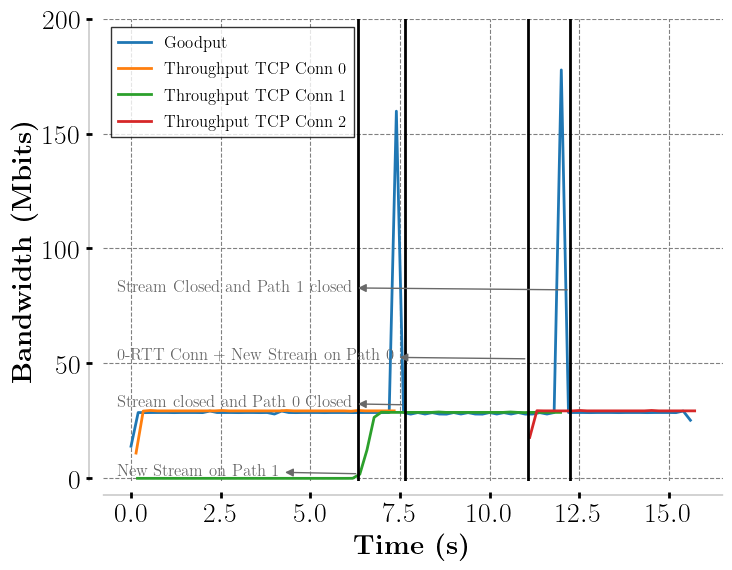
\includegraphics[width=.8\columnwidth]{figures/migration.png}
  \end{center}
  \caption{Application-level connection migration during a 60~MB file download.
    \tcpls temporarily aggregates the two network paths during such a migration.}
  \label{fig:conn_migration}
\end{figure}

\subsection{Bandwidth Aggregation}
\label{sec:bwaggr}
We compare the \tcpls bandwidth aggregation capability to the state-of-the-art
\mptcp.
%To this end, we build a Mininet network~\cite{handigol2012reproducible}
%composed of a client and a server, both dual-stacks. The IPv4 and IPv6 paths
%are
%completely disjoint in this emulated network. Both protocols run in the same
%Mininet topology with two IP paths available, each offering 25Mbps and 10ms
%latency.
Our experiment consists of transferring a 60~MB file over a single path
and enabling the second one after $5$ seconds. \mptcp automatically detects
the new path once we enable the Client's second network interface. For \tcpls,
managing paths is different: the application can use the API to add local or
peer-related addresses at any point of the session. In this experiment, we send
this information after $5$ seconds, create a new \tcp connection to the peer,
and attach a new stream to it. The two streams are coupled together. Our results
appear in Fig.~\ref{fig:multipath_aggregation}. Both protocols aggregate the
two paths and reach a goodput of $\approx$ 50~Mbps.

They have two differences. First, for \mptcp, there is a delay before it becomes fully utilized. This delay is the time required by the Linux kernel
to configure the new network interface IP address, add the required routes, and
finally inform \mptcp~\cite{paasch2012exploring}.
%This explains the time that \mptcp needs to start to use the new path.
Second, \tcpls's aggregated goodput seems less stable than \mptcp. We explain
this discrepancy by the difference of chunk size manipulated by the reordering
algorithms in our experiment: \mptcp reorders packets with a payload of 1,460
bytes, while \tcpls reorders records with the maximum payload size of 16,384 bytes. As concurrent network paths introduce reordering, which is reordered back by both \mptcp and \tcpls, a larger chunk size leads to larger goodput irregularities.

%However, \tcpls might negotiate the record
%size to smooth out this irregularity.
Running the experiment with a record size of 1,500 bytes smooths out the irregularity at a slightly higher CPU cost since encryption and decryption are performed more often. Appendix~\ref{appendix:aggr} shows the results of the same experiment but using a \tls record size of 1,500 bytes instead. With these differences explained, we can conclude that \tcpls offers a bandwidth aggregation service similar to the one offered by state-of-the-art \mptcp.

%Bandwidth aggregation may be useful for some application use-cases. \tcpls's
%strength is to let the application decides whether such a feature would be
%useful for it. This decision may be negotiated at the beginning or dynamically
%during the session.

\begin{figure}[!t]
	\begin{center}
		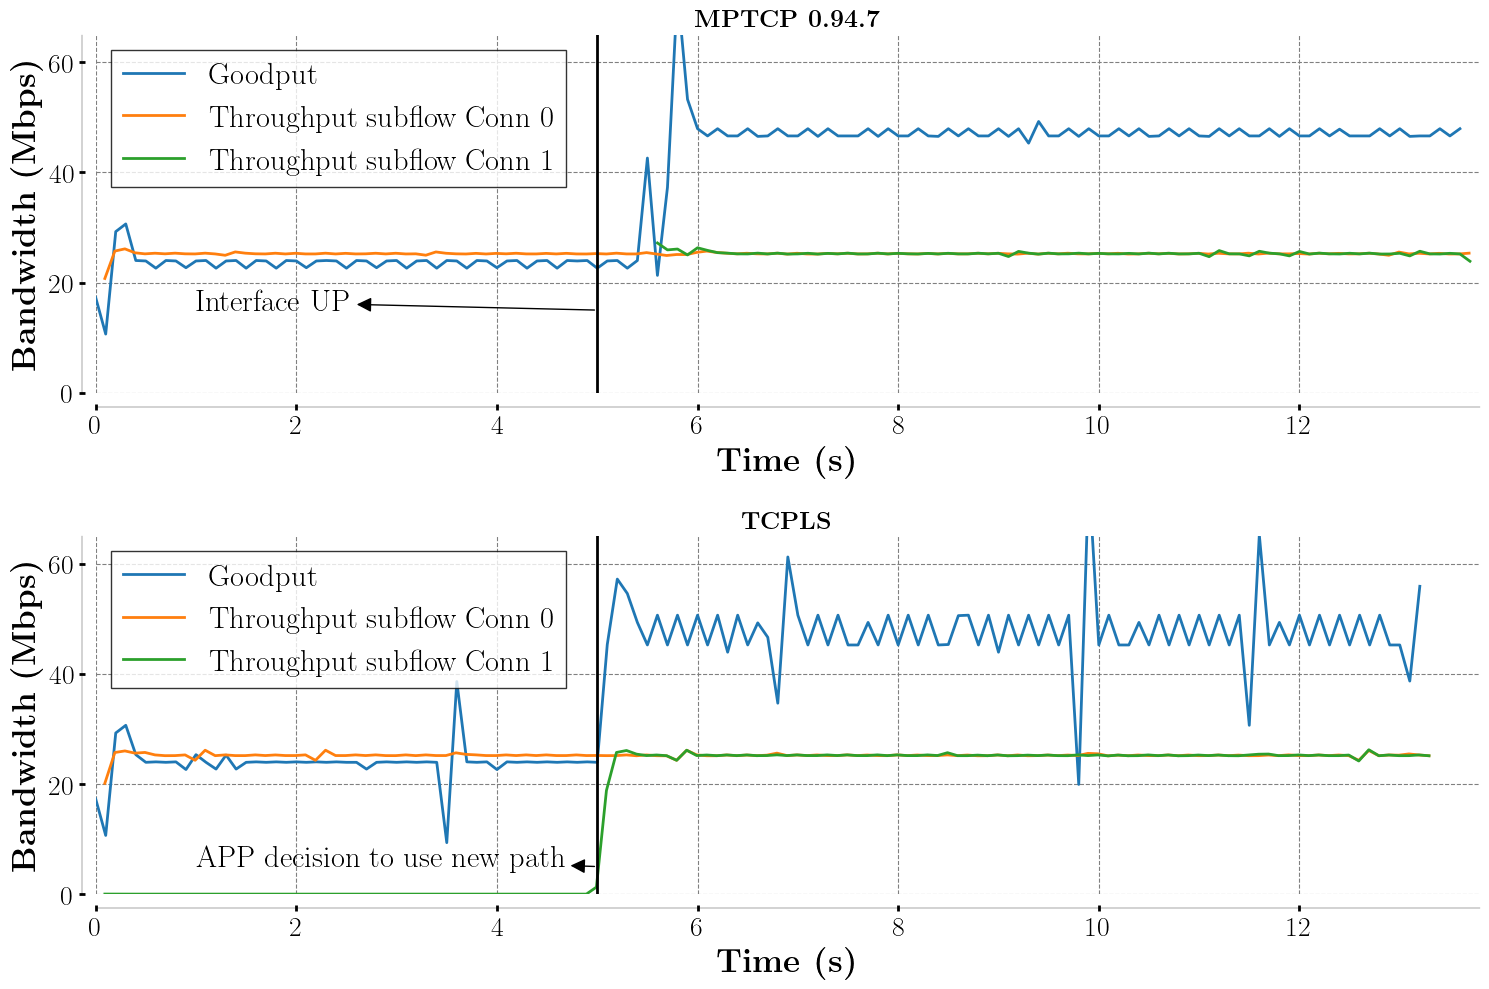
\includegraphics[width=\columnwidth]{figures/aggregate_dual.png}
	\end{center}
	\caption{Bandwidth aggregation comparison between \mptcp (top plot) and
		\tcpls (bottom plot) with a record payload size of 16,384 bytes.}
	\label{fig:multipath_aggregation}
\end{figure}

\subsection{Dynamically Extending \tcpls}
%
%The \tcpls streams enable new use cases. A \tcpls application can
%create and use different streams to carry data. However, since these streams
%are generic, they can also be used by the \tcpls implementation itself to
%exchange control information. To demonstrate the versatility of these control
%streams, we extended \tcpls to enable a server to push a different congestion
%control scheme to a specific client over an existing \tcpls session. Recent
%work on restructuring congestion control has proposed a generic architecture
%for congestion controllers~\cite{narayan2018restructuring}.
%During the last years, the Linux kernel developers have relied on eBPF
%to make the Linux TCP/IP stack~\cite{brakmo2017tcp,tran2020beyond} easier
%to extend. Since Linux kernel version 5.6, an application can inject
%a different congestion control scheme entirely implemented using eBPF. A
%similar
%approach was proposed for \quic in Pluginizing \quic~\cite{de2019pluginizing}.
%We
%leverage these new eBPF capabilities to demonstrate the feasibility of
%injecting
%and updating a congestion control scheme during a \tcpls session.

To illustrate how \tcpls can be dynamically extended, we show how a server can
send an eBPF congestion controller to its client that attaches it in the middle
of a \tcpls session. Fig.~\ref{fig:vegasCubic} reports the goodput obtained
by two \tcpls sessions during a file upload on a Mininet network with a
100~Mbps and 60~ms RTT link.
%We use Mininet over a single 100Mbps emulated link with a
%60msec rtt. Fig.~\ref{fig:vegasCubic} shows a client that uses the \tcp
The orange curve is the first \tcpls session that starts with the Vegas
congestion controller~\cite{brakmo1994tcp}. It rapidly reaches the full capacity of the link. Then, a second \tcpls session, depicted in blue, is
started with the CUBIC congestion controller~\cite{rfc8312}. This quickly
results in an unfair distribution of the bandwidth. The server then sends an
eBPF bytecode implementing the CUBIC congestion controller to the first \tcpls
session which attaches it. The bandwidth distribution becomes fair. We
performed the same experiment for different delays, varying from 10~ms to 100~ms
and obtained similar results.

\begin{figure}[!t]
  \begin{center}
    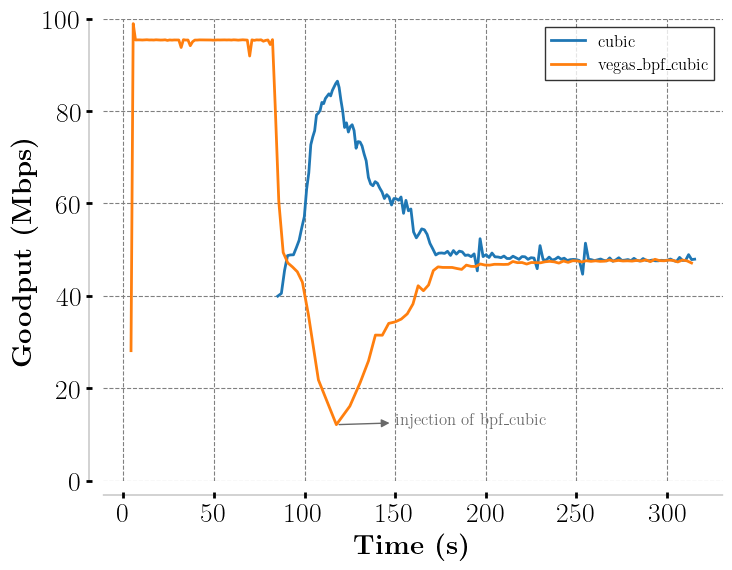
\includegraphics[width=.8\columnwidth]{pretty_plotify/plots/vegas_cubic.png}
  \end{center}
  \caption{\tcpls hosts can exchange eBPF congestion controllers and enable
  them during a \tcpls session.}
  \label{fig:vegasCubic}
\end{figure}
